\documentclass{article}

% if you need to pass options to natbib, use, e.g.:
%     \PassOptionsToPackage{numbers, compress}{natbib}
% before loading neurips_2020

% ready for submission
% \usepackage{neurips_2020}

% to compile a preprint version, e.g., for submission to arXiv, add add the
% [preprint] option:
%     \usepackage[preprint]{neurips_2020}

% to compile a camera-ready version, add the [final] option, e.g.:
%     \usepackage[final]{neurips_2020}

% to avoid loading the natbib package, add option nonatbib:
     \usepackage[nonatbib]{neurips_2020}

\usepackage[utf8]{inputenc} % allow utf-8 input
\usepackage[T1]{fontenc}    % use 8-bit T1 fonts
\usepackage{hyperref}       % hyperlinks
\usepackage{url}            % simple URL typesetting
\usepackage{booktabs}       % professional-quality tables
\usepackage{amsfonts}       % blackboard math symbols
\usepackage{nicefrac}       % compact symbols for 1/2, etc.
\usepackage{microtype}      % microtypography
\usepackage{graphicx}
\usepackage{caption}
\usepackage{subcaption}
\usepackage{amsmath}

\title{Re-evaluation on the BigGAN and SNGAN for image reconstruction with small dataset}

\begin{document}
\nolinenumbers
\maketitle

\begin{abstract}
  In this paper, we propose a re-evaluation on two famous GAN networks for their performance on image generation. Normally, considering the desired output qualities, we will need to train large datasets to obtain meaningful experimental data for further investigation. However, with this amount of data, it is not easy for individuals to complete the training since it needs a huge volume of samples to train over thousands of epochs and the process consumes a huge portion of computing power. In the situation where only limited computing resources are provided, we intend to reassess the two networks, BigGAN and SNGAN, using their pre-trained models, in order to reach some conclusions on which model to choose with limited training samples.
\end{abstract}

\section{Introduction}
    These days, image reconstruction and synthesis have seen their increasing demand in the industry, and quite a lot of generative models are constantly being developed and optimized, but they requirs extremely large datasets to train. To make the process easier, batch statistics adaptation is introduced to reduce the amount of training samples and time needed. 
    
    However, the method is applied on specific GAN models, and the selection on the models has a bearing on the comparative image qualities when images from different classes are trained and tested. Therefore, when there is a limited training samples to be used, it is important to make a wise decision on which model to use for sets of images, and it expands another ground for a research to be conducted.

\section{Related Work}
    Referring to Noguchi et al and recent research outcomes, SNGAN and BigGAN could be two candidates for experiments on image reconstruction with small amount of data. They have their own GAN structures and uniqueness and show distinctive advantages on image generation. In the limited data regimes, Kerras et al proposed an adaptive discriminator augmentation mechanism which can significantly stabilizes the training. This mechanism is proven to be applicable both when training from scratch and when fine-tuning an existing GAN [5]. Wang et al. [7] studied domain adaptation applied to image generation with GAN and concluded that using knowledge from pre-trained networks can shorten the convergence time and improve the quality of generated images when target data size is small. Genin et al. [3] proposed gradient reversal layers for learning domain in variant features. Tzeng et al. [6] focused on studying the correlation between the classes of the source domain and use it to transfer task information. 

\section{Experiments}
    We used the pretrained SNGAN and BigGAN models from author's repository and further trained the scale and shift parameters with three sets of images: flowers, animes and human faces. There are only around 30-50 images for each of them but they represent distinctive characteristics from their own. 
    
    \subsection{Theory}
    Regarding the scale and shift parameters, they are both trainable and are the only parameters updated during our training process. Here the two parameters have the following allocation: 
    \begin{center}
        \begin{equation*}
            G_{Adapt}^{(l)}=G^{(l)}\cdot\gamma^{(l)}+\beta^{(l)}
        \end{equation*}
    \end{center}
    where $G^{(l)}$ is the feature representation of the $l^{\text{th}}$ layer of the generator, $G_{Adapt}^{(l)}$ is the feature of the $l^{\text{th}}$ layer after adaptation. $\gamma$ and $\beta$ represent scale and shift coefficient respectively, which are initialized as 1 and 0. Within the generator structure, $\gamma$ infers the activation strength of the filters while $\beta$ serves as the threshold. When they are both large, the corresponding neuron becomes easy to activate while the neurons are less active with small $\gamma$ and $\beta$ values.
    
    \subsection{Training}
    We used the following image data for the BigGAN and SNGAN, where the BigGAN and SNGAN pretrained weights are from the original author's repository. The 50 face images are from FFHQ dataset, 50 anime faces are from the author's repository and we use 32 images as the flower dataset from TF-Flowers.
    
    Our focus is the reconstruction, and for each dataset, we trained for 500, 2000, 5000 iterations. For two models, the generators are trained using the supervised learning. Similar to Noguchi et al, we used the model embedding method to estimate the latent variable for all training data such that the generated data is close to the images in the training dataset. 
    
    The loss is defined as the following, and we use SGD to update
    \begin{center}
        \begin{align*}
            \text{L1 Loss} & = \sum\limits_i \frac{1}{c_xh_x\omega_x} ||x_i-G_{Adapt}(z_i+\epsilon)||\\
            % \text{L2 Loss} & = \sum\limits_i \frac{1}{c_xh_x\omega_x} ||x_i-G_{Adapt}(z_i+\epsilon)||^2 \\
            \text{Perceptual Loss} & = \sum\limits_i\sum\limits_{l\in layers} \frac{\lambda_C^l}{c_lh_l\omega_l} ||C^{(l)}(x_i)-C^{(l)}(G_{Adapt}(z_i+\epsilon))|| \\
            \textbf{Loss} & = \text{L1 Loss} + \text{Perceptual Loss} \\
            % \textbf{Loss} & = \text{L2 Loss} + \text{Perceptual Loss}
        \end{align*}
    \end{center}
    
    \subsection{Evaluation}
    We use Frechet Inception Distance (FID) and Kernel Maximum Mean Distance (KMMD) for as evaluation metrics. For each dataset, we calculated the FIDs and KMMDs of reconstructed results for iterations 500, 2000, 5000.
    
    \subsubsection{FID}
    The Frechet Inception Distance is a metric that calculates the distance between feature vectors calculated for real and generated images, and lowers scores indicate higher level of similarity. We used \verb+fid_score+ in scipy package to calculate the values. The input and reconstructed images are parsed into the calculation method in batches and corresponding FID scores will be printed.
    
    \subsubsection{KMMD}
    Kernel Maximum Mean Discrepancy measures how similar two distributions are. in the context of image generation via GAN, it evaluates the correlation between the original images and the generated ones. Like FID, a lower KMMD indicates a better generated result. We use a Gaussian kernel for the calculation and use \texttt{kmmd} in thr package \texttt{kernlab} of R to do the implementation.
    

\section{Results}
We tested two models, BigGan and SNGAN for training with different numbers of iterations: 500, 2000, and 5000 with two scales: FID and KMMD. The FID test simply has FID scores as test results, and the KMMD test consists of the following components:
\begin{enumerate}
    \setlength\itemsep{0.01mm}
    \item Hypothesis test with null hypothesis: two images come from the same distribution [8]
    \item Mean and median of 1st and 3rd ordered KMMD scores for input and output images
\end{enumerate}
The FID and KMMD test results are listed in the following two subsections. For detailed illustration of KMMD, such as distribution of KMMD T-test statistics and null hypothesis acceptance and rejection comparison, please read figures in the appendix section.
\subsection{FID}
The tables of FID scores gained by two models trained with different numbers of iterations on different datasets are drawn. Please see the \textbf{Appendix} for table 1, 2, 3


Three tables show that, generally speaking, the FID scores of BigGan are much higher than those of SNGAN, even if in a few cases SNGAN gains higher FID score, but only slightly higher than that gained by BigGAN score. Therefore, from the perspective of FID, the SNGAN is more likely to produce high-quality result compared to BigGAN.

The changing trend of FID scores for two models are invariant with respect to datasets as the iteration number increases. For the SNGAN model, the FID score decreases as the iteration number increases for all three datasets. This decreasing trend is mild on the anime dataset, but rapid on the face dataset.

For the BigGAN model, the FID score decreases initially when iteration number increases from 500 to 2000, and then slightly increases when the iteration number increases from 2000 to 5000. This decreasing trend is mild on the flower dataset, but rapid on the face and anime dataset.

\subsection{KMMD}
Please refer to \textbf{Appendix} for table 4, 5, 6 for KMMD hypothesis test $H_0$ acceptance rates on three datasets, and table 7, 8, 9 for 1st and 3rd mean and median KMMD statistics  on three datasets.

The tables of KMMD statistics gained by two models trained with different numbers of iterations on different datasets are displayed below. The KMMD statistics include the null hypothesis acceptance rate, the mean and the median of first and third order KMMD test statistics. The null hypothesis in the KMMD hypothesis test is that two models are from the same distribution. We reject the null hypothesis when the probabilities computed from the two sample T-test with the KMMD statistics in the tables 7, 8, 9 are lower than the significance level, $\alpha = 0.05$. The less possible the null hypothesis rejected, the more probable the model can generate the high-quality output.

Because of the package implementation, the test function \texttt{kmmd} outputs the KMMD statistics, which is used for the hypothesis two sample T-test, rather than the KMMD scores. Therefore, the higher the KMMD statistics, the less possible the null hypothesis is rejected, hence the more probable the model can generate the high-quality output. The two sample T-test statistics is related to the null hypothesis acceptance rate, the higher the T-test statistics, the harder the null hypothesis is rejected.

There are first and third order statistics, they are computed in different ways, but they have the same result for the two sample T-test.

The tables show that, in general, the images generated by BigGAN are more possible to pass the KMMD test than SNGAN. Since the null hypothesis acceptance rates and mean and median KMMD statiscs of BigGAN are generally higher (sometimes much higher) than those of SNGAN (there is only one case the SNGAN derives outputs with higher acceptance rate and KMMD statistics than BigGAN). Hence, the BigGAN model may generate images with closer distribution to the original images than SNGAN.

For the flower dataset, the acceptance rates (and the test statistics) of both models decrease as the iteration number increases. The test results from the face dataset are not ideal, since the acceptance rates for all cases are nearly 0, and the test statistics for both models decrease as the number of iteration increases, this means the performance on KMMD is even worse as the model is trained more. For the anime dataset, the null hypothesis acceptance rate and test statistics for both models decrease at first, and then increase as the iteration number increases. The acceptance rate  and test statistics of BigGAN increases even more significantly than SNGAN. Therefore, the distribution of output images generated by both models may depend on the distribution of input images.

\section{Conclusion}
    In our research, we compared and analyzed the performance of SNGAN and BigGAN for image reconstruction on three datasets. Our results show that, with the help of the batch statistics adaptation, the shift and scale parameters are tuned. The SNGAN and BigGAN could both generate high-quality reconstructed images by further training the models with small amount of source images. Observing the outputs of two evaluation metrics, it suggests that SNGAN yields results with better qualities evaluated by FID, while BigGAN outperforms SNGAN with KMMD being the quantified indicator.
    
    By visual judgment on the reconstructed results, SNGAN is the winning candidate over BigGAN under fixed iterations. SNGAN generated more visually plausible outcomes at higher iterations since the outlines and contours of the target objects are clearer and more semantically interpretable.
    
\section{Attributions}
    Zhuoheng Huang completed the experiment workflow implementation including the code structure, experiments outline and etc. He also refactored the BigGAN implementation, implemented part of the FID calculation method as well as helped train and obtain the BigGAN reconstruction.
    
    Junming Zhang looked for models to implement and refactored part of SNGAN and BigGAN to produce images suitable for testing. He also designed and completed the testing part: script of KMMD and FID, and made computations and calculations.
    
    Yuchen Tong has refectored the evaluation function in SNGAN to output images with desired format, and helped train and tested the SNGAN for image reconstruction. He was also responsible for labelling, grouping and formatting before the result evaluation stage.
    
    Please see \\\\
    \textbf{Complete reseach source codes, notebooks, graphs, tables and generated results} \\
    \texttt{https://github.com/JunmingZhang/CSC413\_PROJECT} \\\\
    \textbf{Source codes of refactored GAN models} \\ \texttt{https://github.com/JunmingZhang/BigGAN-image-generation} \\ \texttt{https://github.com/JunmingZhang/SNGAN-image-generation}

\newpage
\section*{References}
[1] Alexander, J.A.\ \& Mozer, M.C.\ (1995) Template-based algorithms for
connectionist rule extraction. In G.\ Tesauro, D.S.\ Touretzky and T.K.\ Leen
(eds.), {\it Advances in Neural Information Processing Systems 7},
pp.\ 609--616. Cambridge, MA: MIT Press.

[2] Bower, J.M.\ \& Beeman, D.\ (1995) {\it The Book of GENESIS: Exploring
  Realistic Neural Models with the GEneral NEural SImulation System.}  New York:
TELOS/Springer--Verlag.

[3] Ganin, Y., Ustinova, E., Ajakan, H., Germain, P., Larochelle, H., Laviolette, F., Marchand, N., Lempitsky, V. (2016) Domain-adversarial training of neural networks. JMLR {\bf{17}} (1), 2096-2030.

[4] Hasselmo, M.E., Schnell, E.\ \& Barkai, E.\ (1995) Dynamics of learning and
recall at excitatory recurrent synapses and cholinergic modulation in rat
hippocampal region CA3. {\it Journal of Neuroscience} {\bf 15}(7):5249-5262.

[5] Karras, T., Aittala, M., Hellsten, J., Laine, S., Lehtinen, J., \& Aila, T. (2020). Training generative adversarial networks with limited data.

[6] Tzeng, E., Hoffman, J., Darrell, T., Saenko, K. (2015) Simultaneous deep transfer across domains and tasks. In: CVPR. pp. 4068-4076.

[7] Wang, Y., Wu, C., Herranz, L.\ \&  Weijer, J. (2018) Transferring GANs: generating images from limited data.

[8] Gretton, A., Borgwardt, K., Rasch, M., Scholkopf, B., Smola, A. (2006) A Kernel Method for the Two-Sample-Problem

\newpage
\section*{Appendix}

\subsection*{Samples generated by SNGAN}
\begin{figure}[h!]
    \caption{Dataset Flower}
     \centering
     \begin{subfigure}[b]{0.24\textwidth}
         \centering
         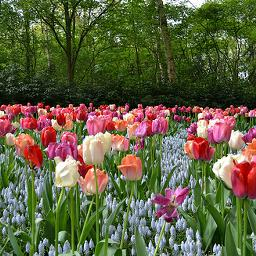
\includegraphics[width=\textwidth]{illustration/flower_input.jpeg}
         \caption{input}
     \end{subfigure}
     \begin{subfigure}[b]{0.24\textwidth}
         \centering
         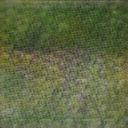
\includegraphics[width=\textwidth]{illustration/flower_sngan_500.jpg}
         \caption{500 iterations}
     \end{subfigure}
     \begin{subfigure}[b]{0.24\textwidth}
         \centering
         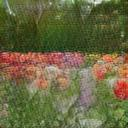
\includegraphics[width=\textwidth]{illustration/flower_sngan_2000.jpg}
         \caption{2000 iterations}
     \end{subfigure}
     \begin{subfigure}[b]{0.24\textwidth}
         \centering
         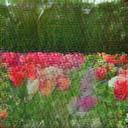
\includegraphics[width=\textwidth]{illustration/flower_sngan_5000.jpg}
         \caption{5000 iterations}
     \end{subfigure}
\end{figure}

\begin{figure}[h!]
    \caption{Dataset Face}
     \centering
     \begin{subfigure}[b]{0.24\textwidth}
         \centering
         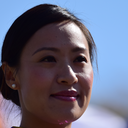
\includegraphics[width=\textwidth]{illustration/face_input.png}
         \caption{input}
     \end{subfigure}
     \begin{subfigure}[b]{0.24\textwidth}
         \centering
         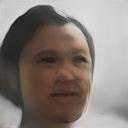
\includegraphics[width=\textwidth]{illustration/face_sngan_500.jpg}
         \caption{500 iterations}
     \end{subfigure}
     \begin{subfigure}[b]{0.24\textwidth}
         \centering
         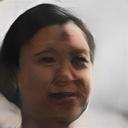
\includegraphics[width=\textwidth]{illustration/face_sngan_2000.jpg}
         \caption{2000 iterations}
     \end{subfigure}
     \begin{subfigure}[b]{0.24\textwidth}
         \centering
         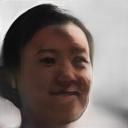
\includegraphics[width=\textwidth]{illustration/face_sngan_5000.jpg}
         \caption{5000 iterations}
     \end{subfigure}
\end{figure}

\begin{figure}[h!]
    \caption{Dataset Anime}
     \centering
     \begin{subfigure}[b]{0.24\textwidth}
         \centering
         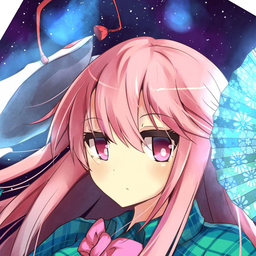
\includegraphics[width=\textwidth]{illustration/anime_input.png}
         \caption{input}
     \end{subfigure}
     \begin{subfigure}[b]{0.24\textwidth}
         \centering
         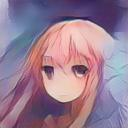
\includegraphics[width=\textwidth]{illustration/anime_sngan_500.jpg}
         \caption{500 iterations}
     \end{subfigure}
     \begin{subfigure}[b]{0.24\textwidth}
         \centering
         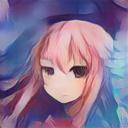
\includegraphics[width=\textwidth]{illustration/anime_sngan_2000.jpg}
         \caption{2000 iterations}
     \end{subfigure}
     \begin{subfigure}[b]{0.24\textwidth}
         \centering
         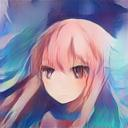
\includegraphics[width=\textwidth]{illustration/anime_sngan_5000.jpg}
         \caption{5000 iterations}
     \end{subfigure}
\end{figure}

\newpage
\subsection*{Samples generated by BigGAN}
\begin{figure}[h!]
    \caption{Dataset Flower}
     \centering
     \begin{subfigure}[b]{0.24\textwidth}
         \centering
         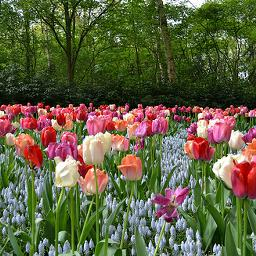
\includegraphics[width=\textwidth]{illustration/flower_input.jpeg}
         \caption{input}
     \end{subfigure}
     \begin{subfigure}[b]{0.24\textwidth}
         \centering
         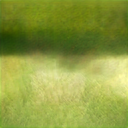
\includegraphics[width=\textwidth]{illustration/flower_biggan_500.png}
         \caption{500 iterations}
     \end{subfigure}
     \begin{subfigure}[b]{0.24\textwidth}
         \centering
         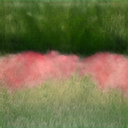
\includegraphics[width=\textwidth]{illustration/flower_biggan_2000.png}
         \caption{2000 iterations}
     \end{subfigure}
     \begin{subfigure}[b]{0.24\textwidth}
         \centering
         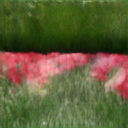
\includegraphics[width=\textwidth]{illustration/flower_biggan_5000.png}
         \caption{5000 iterations}
     \end{subfigure}
\end{figure}

\begin{figure}[h!]
    \caption{Dataset Face}
     \centering
     \begin{subfigure}[b]{0.24\textwidth}
         \centering
         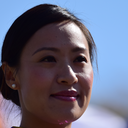
\includegraphics[width=\textwidth]{illustration/face_input.png}
         \caption{input}
     \end{subfigure}
     \begin{subfigure}[b]{0.24\textwidth}
         \centering
         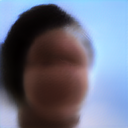
\includegraphics[width=\textwidth]{illustration/face_biggan_500.png}
         \caption{500 iterations}
     \end{subfigure}
     \begin{subfigure}[b]{0.24\textwidth}
         \centering
         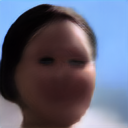
\includegraphics[width=\textwidth]{illustration/face_biggan_2000.png}
         \caption{2000 iterations}
     \end{subfigure}
     \begin{subfigure}[b]{0.24\textwidth}
         \centering
         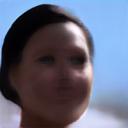
\includegraphics[width=\textwidth]{illustration/face_biggan_5000.png}
         \caption{5000 iterations}
     \end{subfigure}
\end{figure}

\begin{figure}[h!]
    \caption{Dataset Anime}
     \centering
     \begin{subfigure}[b]{0.24\textwidth}
         \centering
         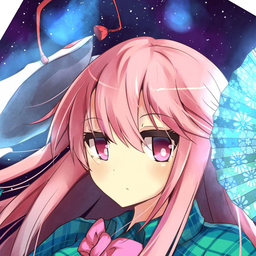
\includegraphics[width=\textwidth]{illustration/anime_input.png}
         \caption{input}
     \end{subfigure}
     \begin{subfigure}[b]{0.24\textwidth}
         \centering
         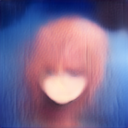
\includegraphics[width=\textwidth]{illustration/anime_biggan_500.png}
         \caption{500 iterations}
     \end{subfigure}
     \begin{subfigure}[b]{0.24\textwidth}
         \centering
         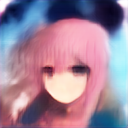
\includegraphics[width=\textwidth]{illustration/anime_biggan_2000.png}
         \caption{2000 iterations}
     \end{subfigure}
     \begin{subfigure}[b]{0.24\textwidth}
         \centering
         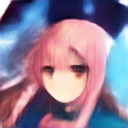
\includegraphics[width=\textwidth]{illustration/anime_biggan_5000.png}
         \caption{5000 iterations}
     \end{subfigure}
\end{figure}

\newpage
\subsection*{FID scores of three datasets by models}
\begin{table}[h!]
 \centering
 \caption{FID scores on dataset flower}
 \begin{tabular}{||c | c | c | c||}
 \hline
 & 500 iterations & 2000 iterations & 5000 iterations \\ [0.5ex] 
 \hline\hline
 SNGAN & 332.54 & 254.81 & 222.53 \\ 
 \hline
 BigGAN & 354.25 & 297.03 & 302.93 \\
 \hline
\end{tabular}
\end{table}

\begin{table}[h!]
\centering
\caption{FID scores on dataset face}
 \begin{tabular}{||c | c | c | c||} 
 \hline
 & 500 iterations & 2000 iterations & 5000 iterations \\ [0.5ex] 
 \hline\hline
 SNGAN & 336.60 & 226.01 & 218.61 \\ 
 \hline
 BigGAN & 331.01 & 220.89 & 260.48 \\
 \hline
\end{tabular}
\end{table}

\begin{table}[h!]
\centering
\caption{FID scores on dataset anime}
 \begin{tabular}{||c | c | c | c||} 
 \hline
 & 500 iterations & 2000 iterations & 5000 iterations \\ [0.5ex] 
 \hline\hline
 SNGAN & 201.42 & 187.98 & 182.03 \\ 
 \hline
 BigGAN & 284.15 & 188.65 & 242.54 \\
 \hline
\end{tabular}
\end{table}


\subsection*{KMMD hypothesis test $H_0$ acceptance rates of three datasets by models}
\begin{table}[h!]
\centering
\caption{KMMD hypothesis test $H_0$ acceptance rates on dataset flower}
 \begin{tabular}{||c | c | c | c||} 
 \hline
 & 500 iterations & 2000 iterations & 5000 iterations \\ [0.5ex] 
 \hline\hline
 SNGAN & 0.75 & 0.50 & 0.25 \\ 
 \hline
 BigGAN & 0.84 & 0.56 & 0.31 \\
 \hline
\end{tabular}
\end{table}

\begin{table}[h!]
\centering
\caption{KMMD hypothesis test $H_0$ acceptance rates on dataset face}
 \begin{tabular}{||c | c | c | c||} 
 \hline
 & 500 iterations & 2000 iterations & 5000 iterations \\ [0.5ex] 
 \hline\hline
 SNGAN & 0.00 & 0.02 & 0.00 \\ 
 \hline
 BigGAN & 0.04 & 0.00 & 0.00 \\
 \hline
\end{tabular}
\end{table}

\begin{table}[h!]
\centering
\caption{KMMD hypothesis test $H_0$ acceptance rates on dataset anime}
 \begin{tabular}{||c | c | c | c||} 
 \hline
 & 500 iterations & 2000 iterations & 5000 iterations \\ [0.5ex] 
 \hline\hline
 SNGAN & 0.30 & 0.12 & 0.18 \\ 
 \hline
 BigGAN & 0.50 & 0.16 & 0.84 \\
 \hline
\end{tabular}
\end{table}


\subsection*{1st and 3rd mean and median KMMD statistics of three datasets by models}
\begin{table}[hbt!]
\centering
\caption{1st and 3rd mean and median KMMD statistics on dataset flower}
 \begin{tabular}{||c | c | c | c||} 
 \hline
 & 500 iterations & 2000 iterations & 5000 iterations \\ [0.5ex] 
 \hline\hline
 SNGAN 1st order & 0.4678, 0.4767 & 0.3525, 0.3428 & 0.2732, 0.2450 \\ 
 \hline
 SNGAN 3rd order & 0.2376, 0.2246 & 0.1400, 0.1149 & 0.0931, 0.0581 \\ 
 \hline
 BigGAN 1st order & 0.5321, 0.4479 & 0.4120, 0.4007 & 0.2999, 0.2525 \\
 \hline
 BigGAN 3rd order & 0.3171, 0.1972 & 0.2063, 0.1575 & 0.1196, 0.0620 \\
 \hline
\end{tabular}
\end{table}

\begin{table}[hbt!]
\centering
\caption{1st and 3rd mean and median KMMD statistics on dataset face}
 \begin{tabular}{||c | c | c | c||} 
 \hline
 & 500 iterations & 2000 iterations & 5000 iterations \\ [0.5ex] 
 \hline\hline
 SNGAN 1st order & 0.2525, 0.2429 & 0.2082, 0.2037 & 0.1949, 0.1852 \\ 
 \hline
 SNGAN 3rd order & 0.0660, 0.0558 & 0.0459, 0.0390 & 0.0400, 0.0323 \\ 
 \hline
 BigGAN 1st order & 0.2749, 0.2501 & 0.1789, 0.1657 & 0.1377, 0.1240 \\
 \hline
 BigGAN 3rd order & 0.0817, 0.0587 & 0.0329, 0.0255 & 0.0205, 0.0138 \\
 \hline
\end{tabular}
\end{table}

\begin{table}[hbt!]
\centering
\caption{1st and 3rd mean and median KMMD statistics on dataset anime}
 \begin{tabular}{||c | c | c | c||} 
 \hline
 & 500 iterations & 2000 iterations & 5000 iterations \\ [0.5ex] 
 \hline\hline
 SNGAN 1st order & 0.2923, 0.2832 & 0.2372, 0.2326 & 0.2537, 0.2542 \\ 
 \hline
 SNGAN 3rd order & 0.0920, 0.0781 & 0.0613, 0.0523 & 0.0688, 0.0630 \\ 
 \hline
 BigGAN 1st order & 0.3319, 0.3414 & 0.2367, 0.2156 & 0.6939, 0.6815 \\
 \hline
 BigGAN 3rd order & 0.1165, 0.1140 & 0.0604, 0.0444 & 0.5035, 0.4570 \\
 \hline
\end{tabular}
\end{table}

\pagebreak
\subsection*{Null hypothesis reject vs cannot reject for SNGAN}
\begin{figure}[h!]
    \caption{Dataset Flower}
     \centering
     \begin{subfigure}[b]{0.3\textwidth}
         \centering
         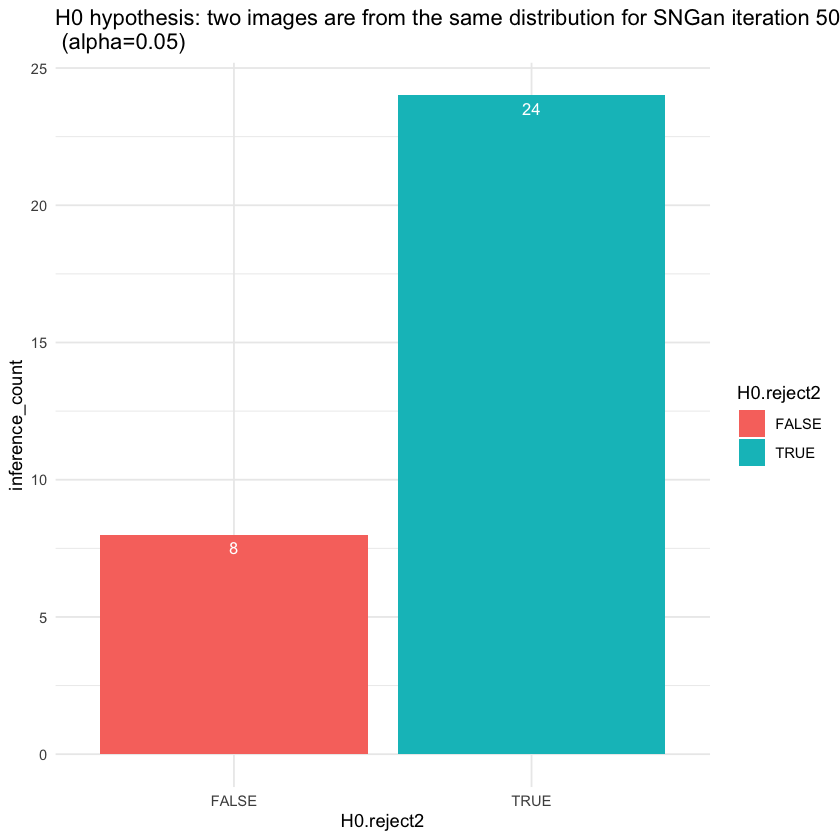
\includegraphics[width=\textwidth]{kmmd_figures/sngan_flower_500.png}
         \caption{500 iterations}
     \end{subfigure}
     \hfill
     \begin{subfigure}[b]{0.3\textwidth}
         \centering
         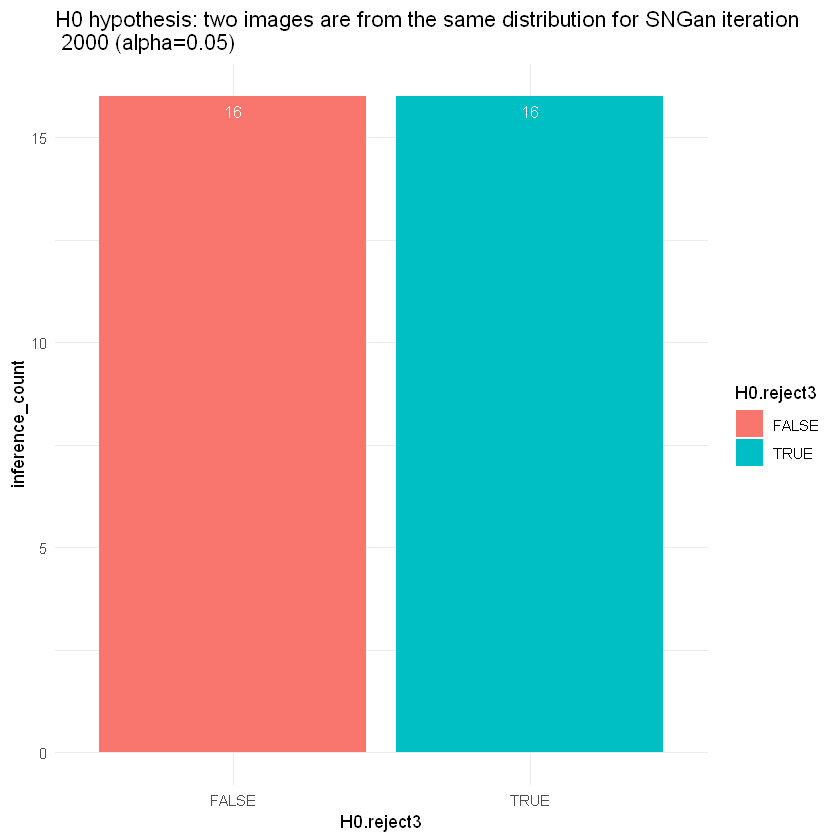
\includegraphics[width=\textwidth]{kmmd_figures/sngan_flower_2000.png}
         \caption{2000 iterations}
     \end{subfigure}
     \hfill
     \begin{subfigure}[b]{0.3\textwidth}
         \centering
         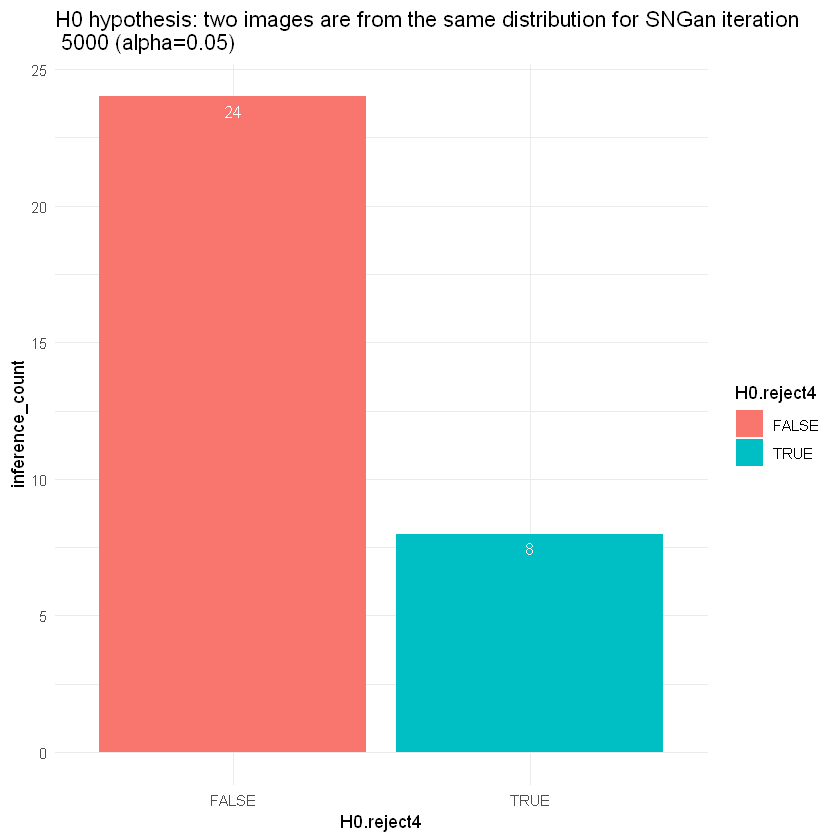
\includegraphics[width=\textwidth]{kmmd_figures/sngan_flower_5000.png}
         \caption{5000 iterations}
     \end{subfigure}
\end{figure}

\begin{figure}[h!]
    \caption{Dataset Face}
     \centering
     \begin{subfigure}[b]{0.3\textwidth}
         \centering
         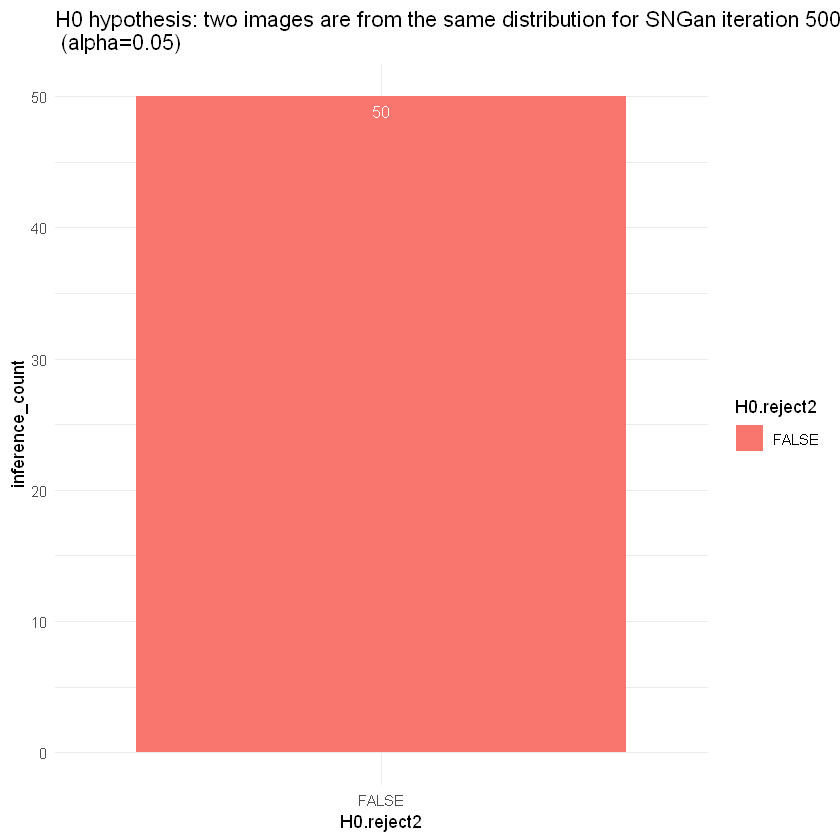
\includegraphics[width=\textwidth]{kmmd_figures/sngan_face_500.png}
         \caption{500 iterations}
     \end{subfigure}
     \hfill
     \begin{subfigure}[b]{0.3\textwidth}
         \centering
         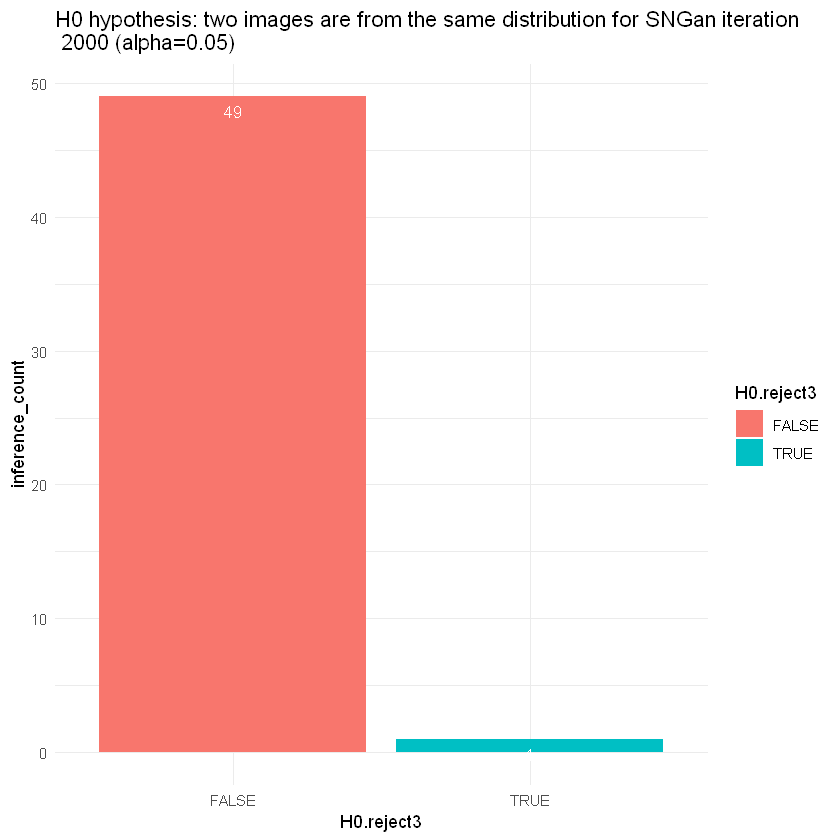
\includegraphics[width=\textwidth]{kmmd_figures/sngan_face_2000.png}
         \caption{2000 iterations}
     \end{subfigure}
     \hfill
     \begin{subfigure}[b]{0.3\textwidth}
         \centering
         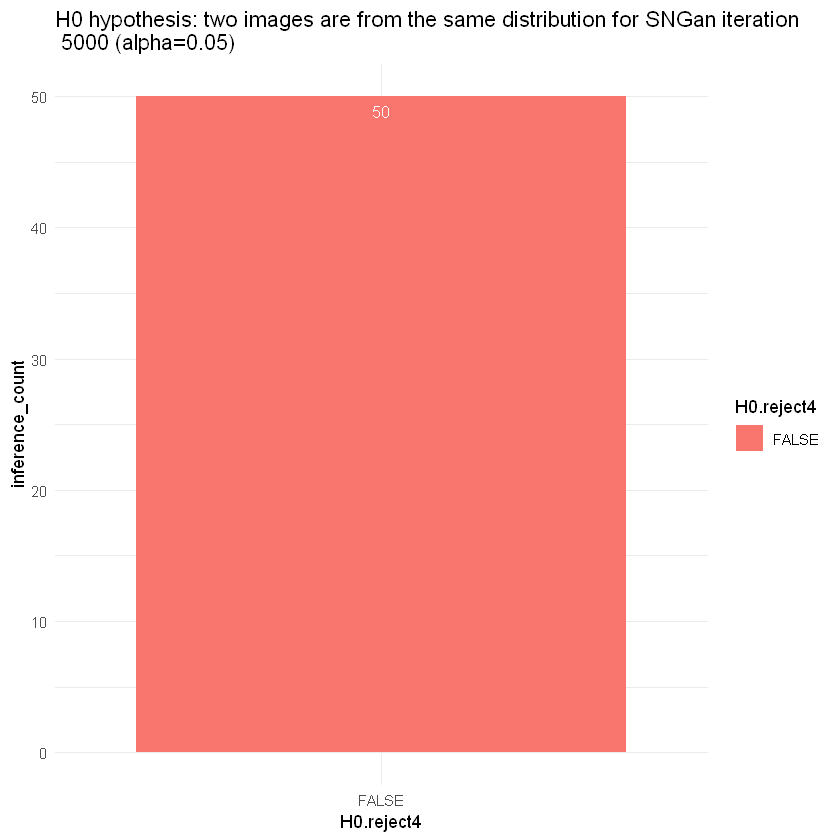
\includegraphics[width=\textwidth]{kmmd_figures/sngan_face_5000.png}
         \caption{5000 iterations}
     \end{subfigure}
\end{figure}

\begin{figure}[h!]
    \caption{Dataset Anime}
     \centering
     \begin{subfigure}[b]{0.3\textwidth}
         \centering
         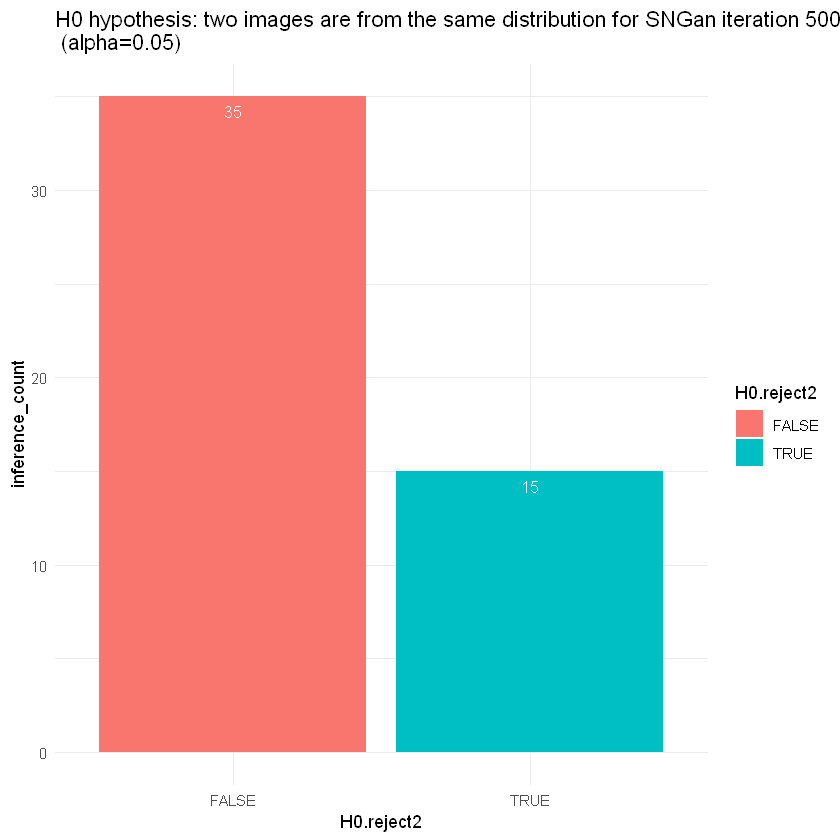
\includegraphics[width=\textwidth]{kmmd_figures/sngan_anime_500.png}
         \caption{500 iterations}
     \end{subfigure}
     \hfill
     \begin{subfigure}[b]{0.3\textwidth}
         \centering
         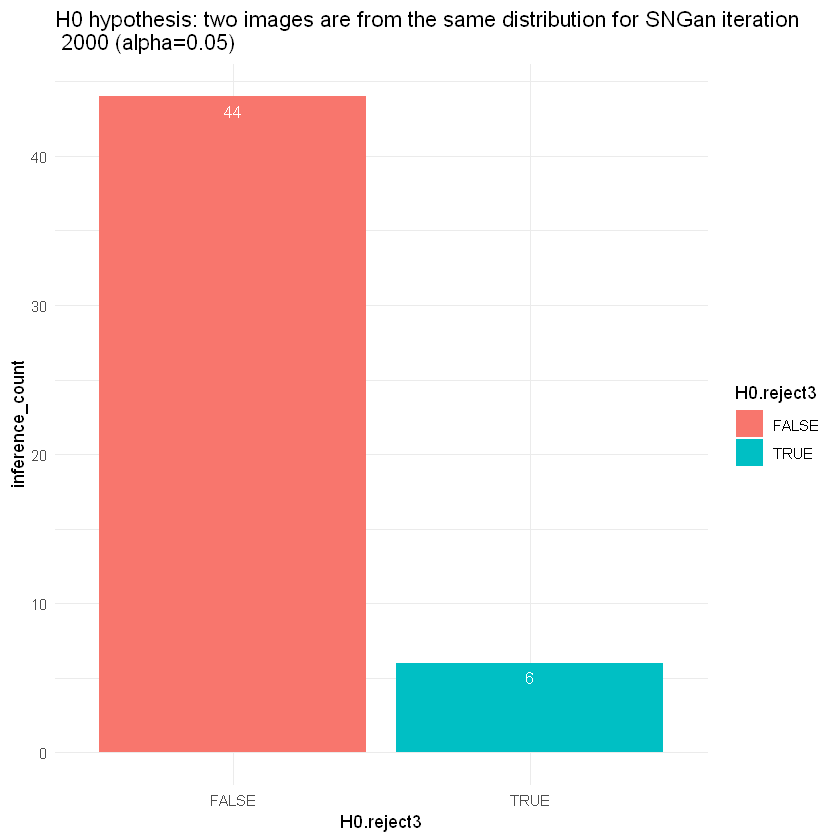
\includegraphics[width=\textwidth]{kmmd_figures/sngan_anime_2000.png}
         \caption{2000 iterations}
     \end{subfigure}
     \hfill
     \begin{subfigure}[b]{0.3\textwidth}
         \centering
         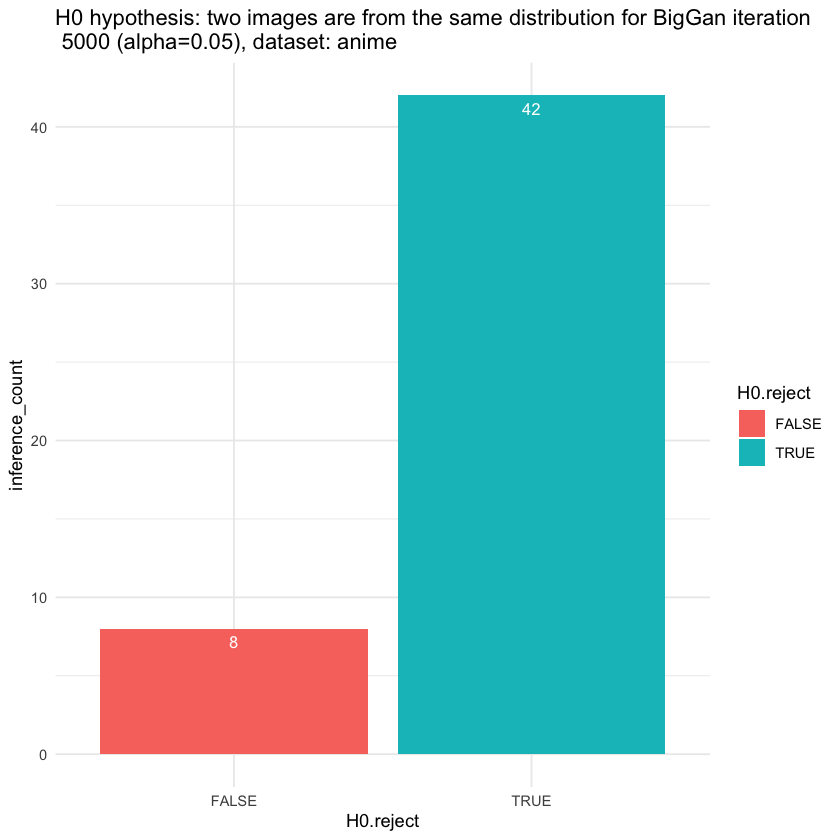
\includegraphics[width=\textwidth]{kmmd_figures/biggan_anime_5000.png}
         \caption{5000 iterations}
     \end{subfigure}
\end{figure}

\newpage
\subsection*{Null hypothesis reject vs cannot reject for BigGAN}

\begin{figure}[h!]
    \caption{Dataset Flower}
     \centering
     \begin{subfigure}[b]{0.3\textwidth}
         \centering
         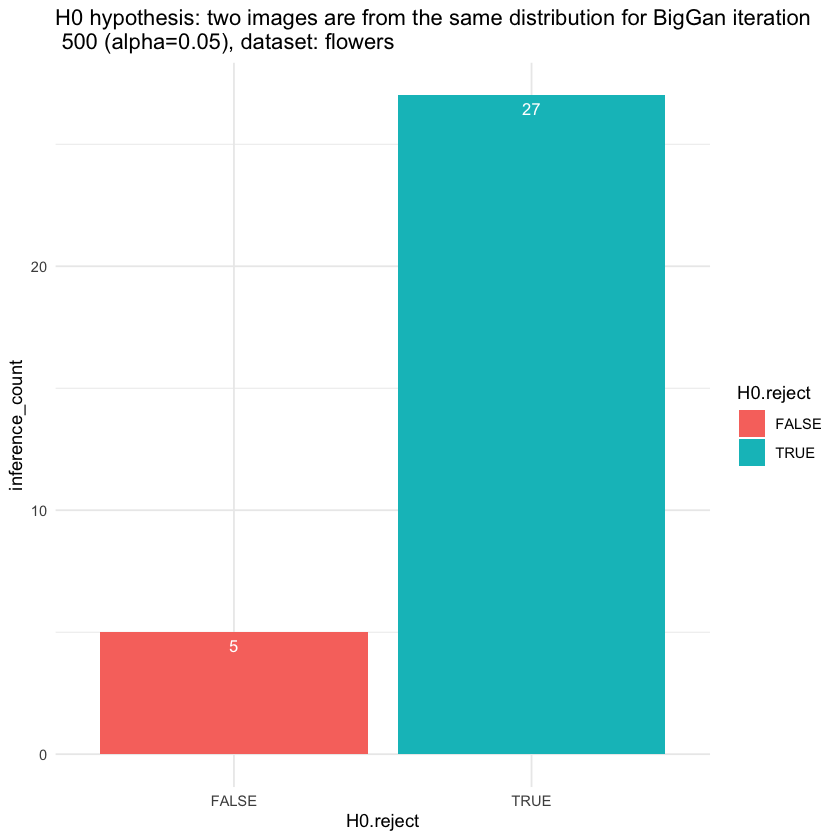
\includegraphics[width=\textwidth]{kmmd_figures/biggan_flower_500.png}
         \caption{500 iterations}
     \end{subfigure}
     \hfill
     \begin{subfigure}[b]{0.3\textwidth}
         \centering
         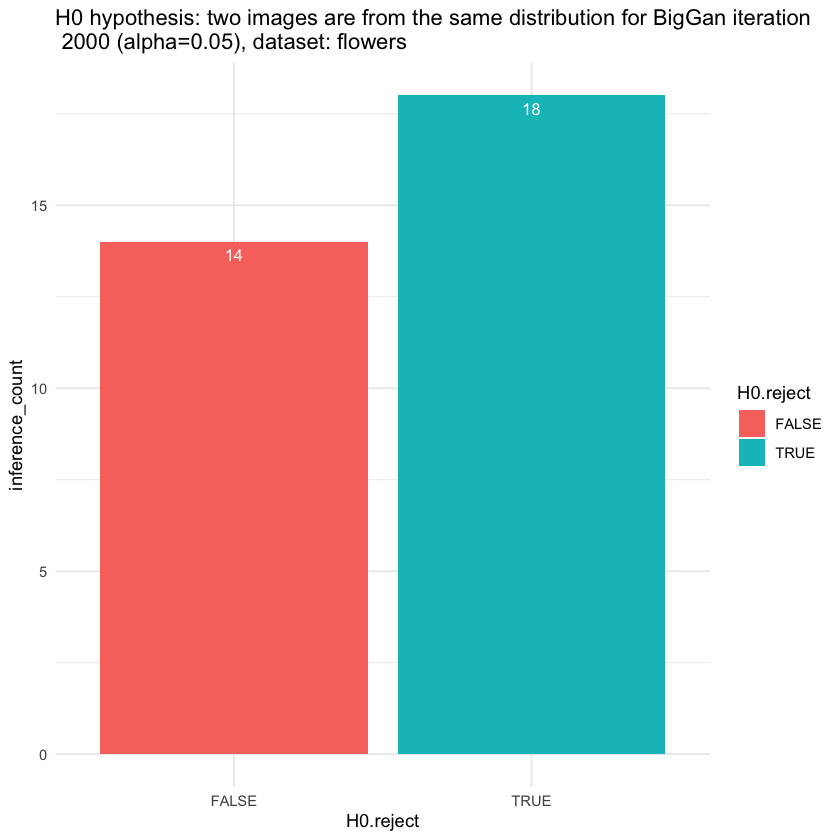
\includegraphics[width=\textwidth]{kmmd_figures/biggan_flower_2000.png}
         \caption{2000 iterations}
     \end{subfigure}
     \hfill
     \begin{subfigure}[b]{0.3\textwidth}
         \centering
         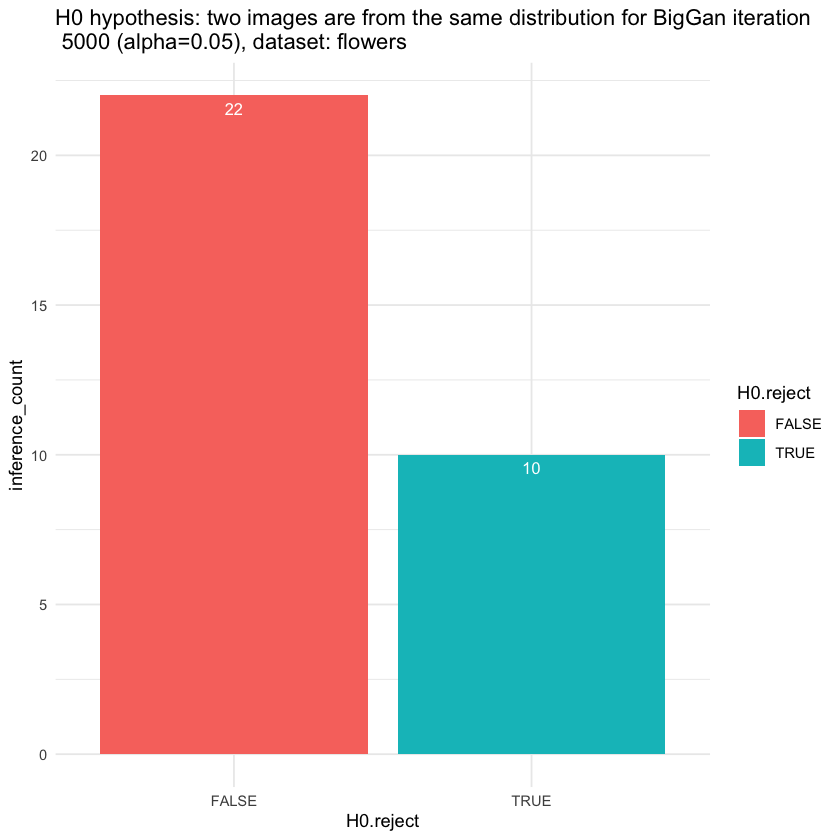
\includegraphics[width=\textwidth]{kmmd_figures/biggan_flower_5000.png}
         \caption{5000 iterations}
     \end{subfigure}
\end{figure}

\begin{figure}[h!]
    \caption{Dataset Face}
     \centering
     \begin{subfigure}[b]{0.3\textwidth}
         \centering
         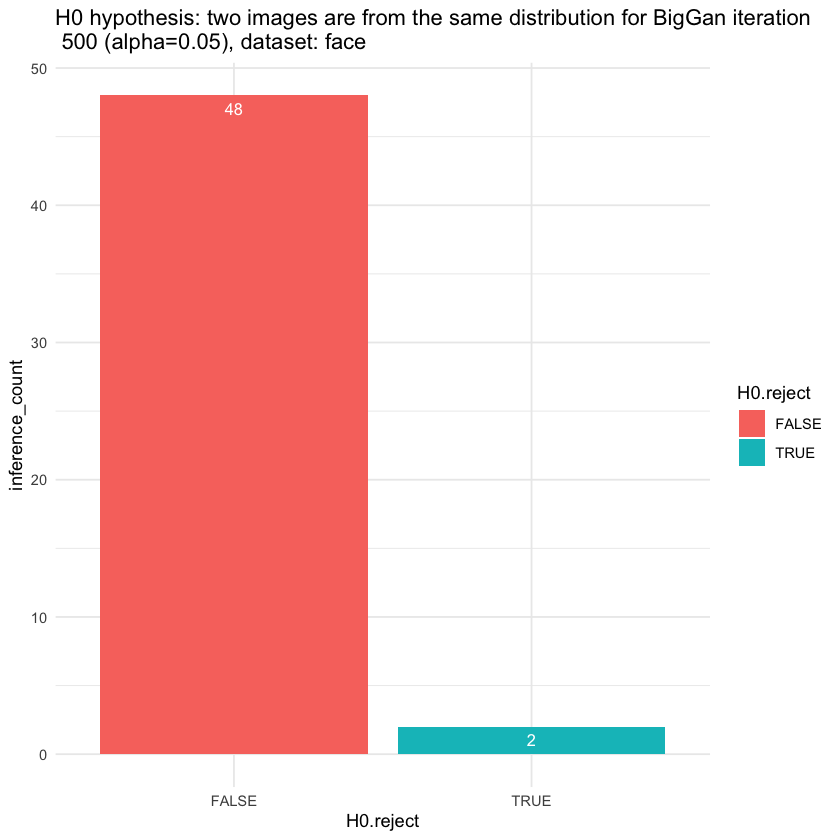
\includegraphics[width=\textwidth]{kmmd_figures/biggan_face_500.png}
         \caption{500 iterations}
     \end{subfigure}
     \hfill
     \begin{subfigure}[b]{0.3\textwidth}
         \centering
         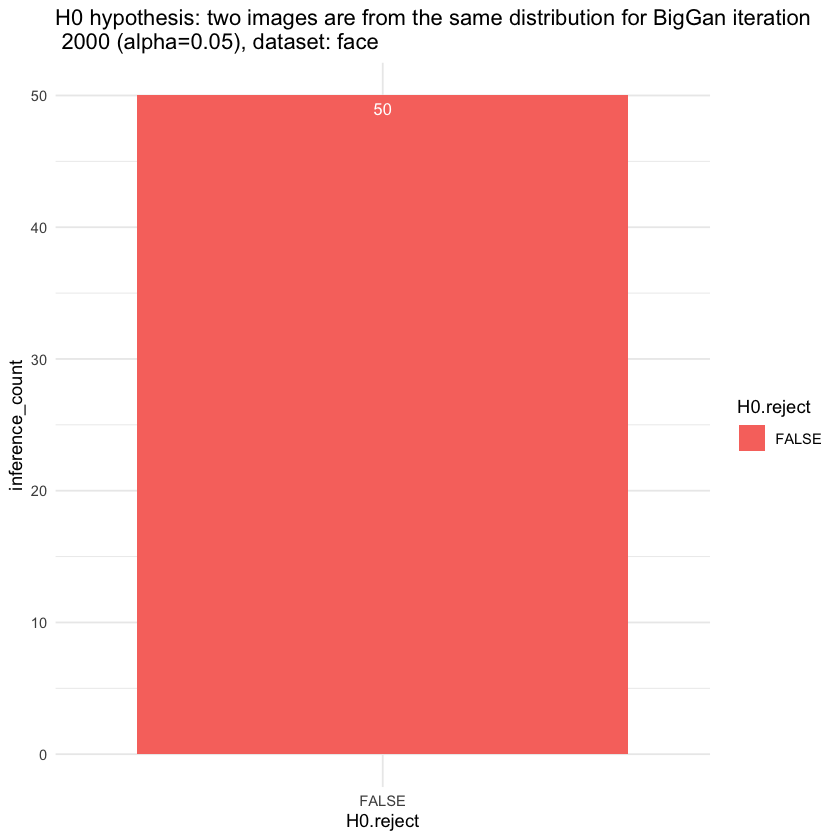
\includegraphics[width=\textwidth]{kmmd_figures/biggan_face_2000.png}
         \caption{2000 iterations}
     \end{subfigure}
     \hfill
     \begin{subfigure}[b]{0.3\textwidth}
         \centering
         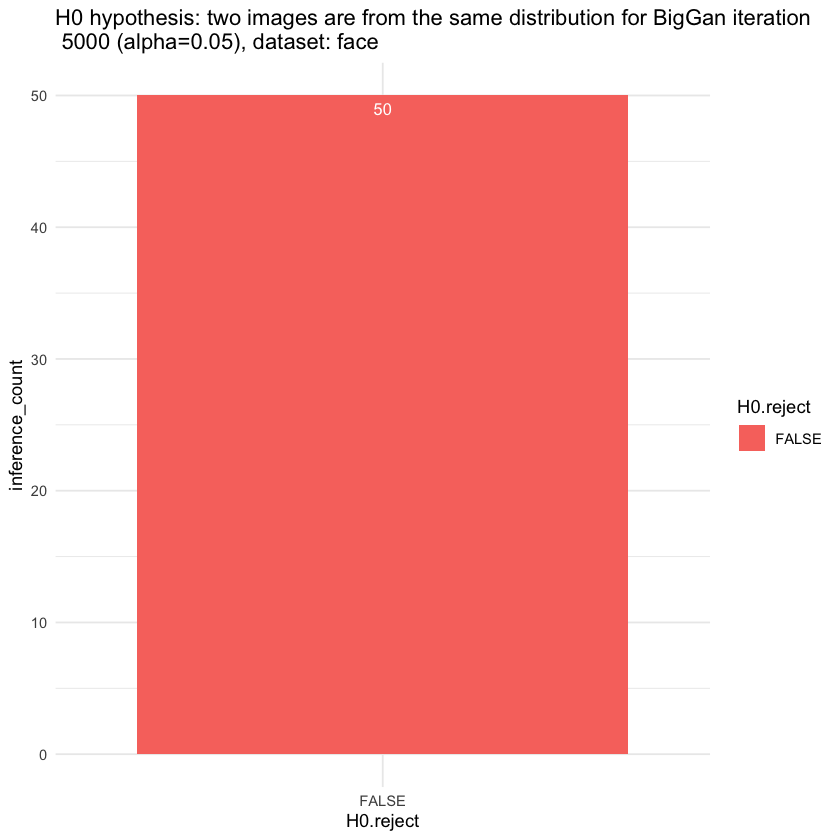
\includegraphics[width=\textwidth]{kmmd_figures/biggan_face_5000.png}
         \caption{5000 iterations}
     \end{subfigure}
\end{figure}

\begin{figure}[h!]
    \caption{Dataset Anime}
     \centering
     \begin{subfigure}[b]{0.3\textwidth}
         \centering
         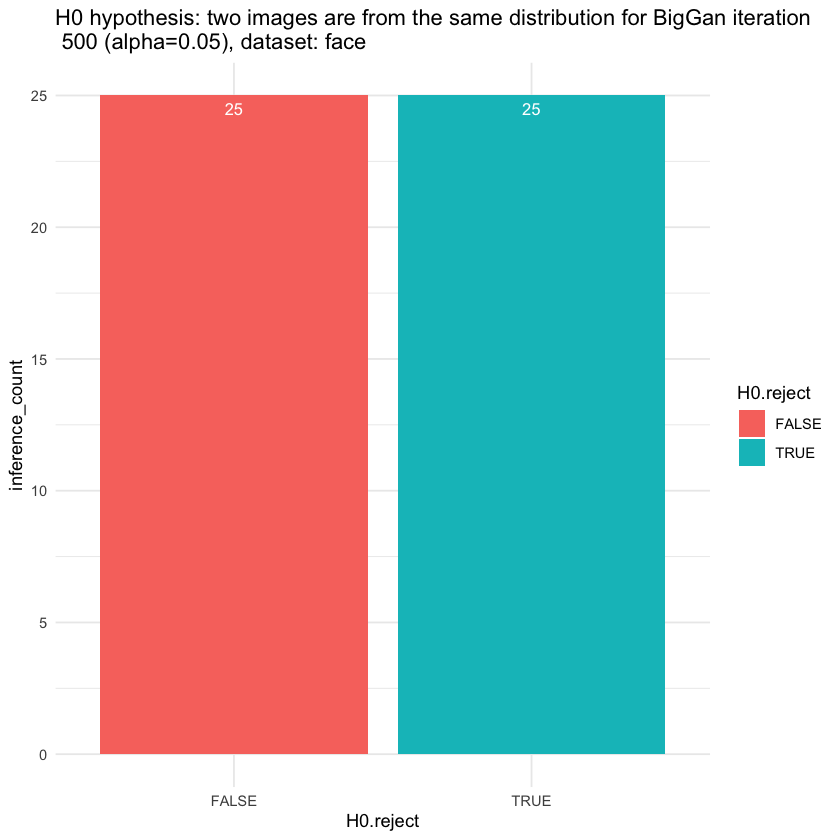
\includegraphics[width=\textwidth]{kmmd_figures/biggan_anime_500.png}
         \caption{500 iterations}
     \end{subfigure}
     \hfill
     \begin{subfigure}[b]{0.3\textwidth}
         \centering
         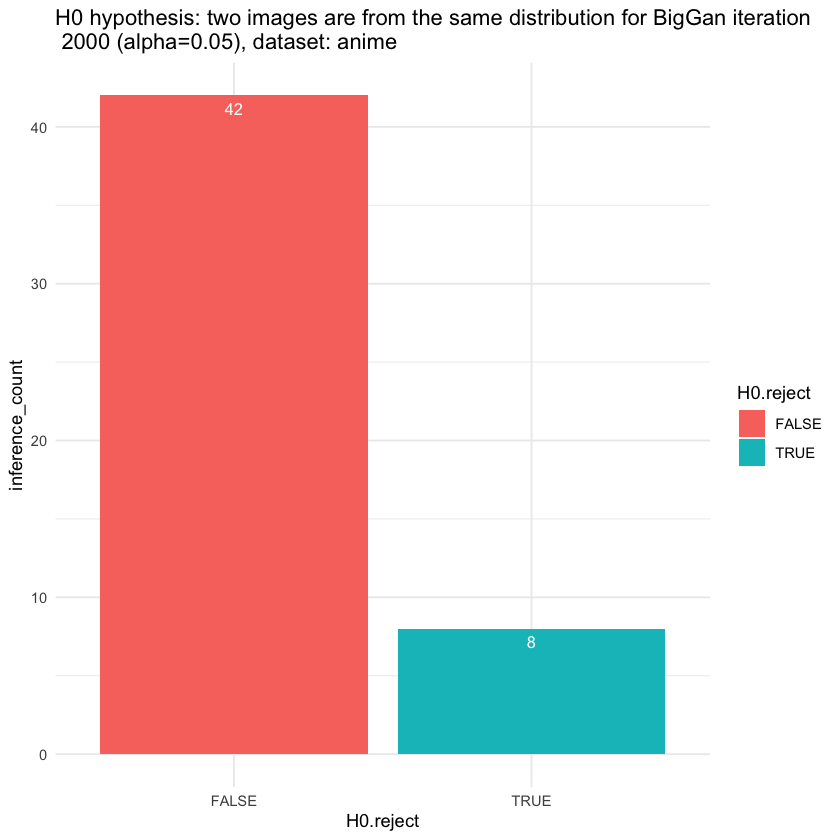
\includegraphics[width=\textwidth]{kmmd_figures/biggan_anime_2000.png}
         \caption{2000 iterations}
     \end{subfigure}
     \hfill
     \begin{subfigure}[b]{0.3\textwidth}
         \centering
         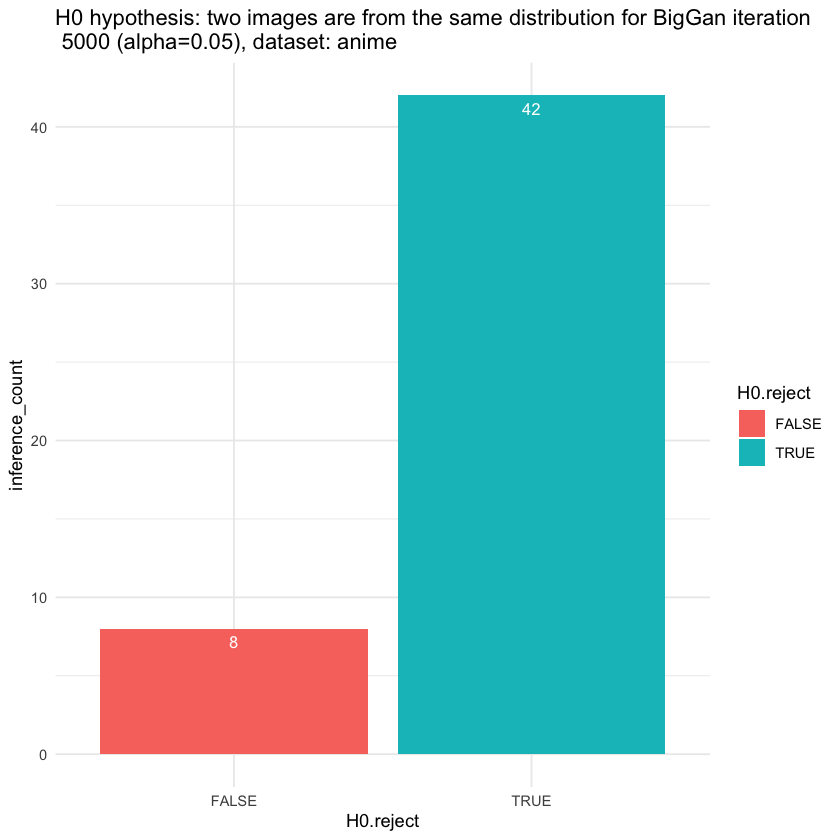
\includegraphics[width=\textwidth]{kmmd_figures/biggan_anime_5000.png}
         \caption{5000 iterations}
     \end{subfigure}
\end{figure}

\newpage
\subsection*{KMMD first order test statistics distribution for SNGAN}
\begin{figure}[h!]
    \caption{Dataset Flower}
     \centering
     \begin{subfigure}[b]{0.3\textwidth}
         \centering
         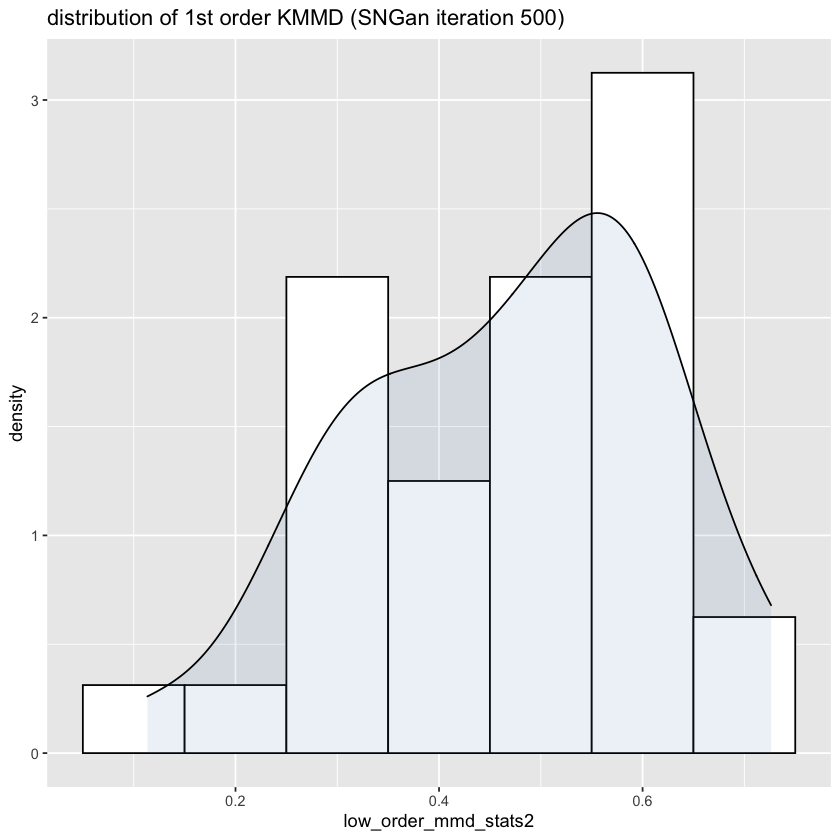
\includegraphics[width=\textwidth]{kmmd_figures/sngan_flower_lowdist_500.png}
         \caption{500 iterations}
     \end{subfigure}
     \hfill
     \begin{subfigure}[b]{0.3\textwidth}
         \centering
         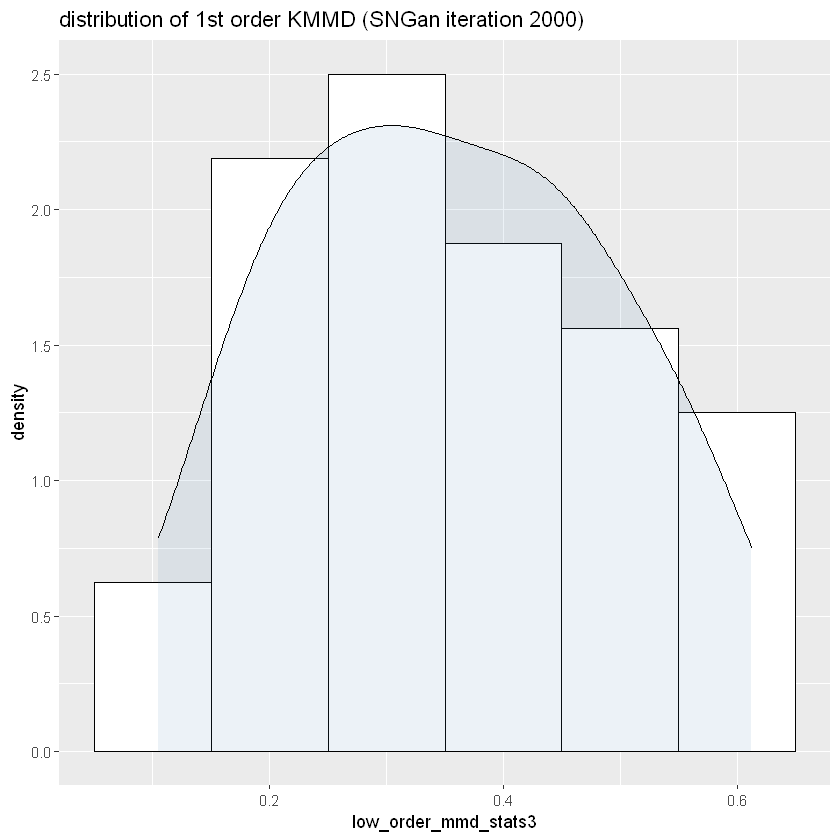
\includegraphics[width=\textwidth]{kmmd_figures/sngan_flower_lowdist_2000.png}
         \caption{2000 iterations}
     \end{subfigure}
     \hfill
     \begin{subfigure}[b]{0.3\textwidth}
         \centering
         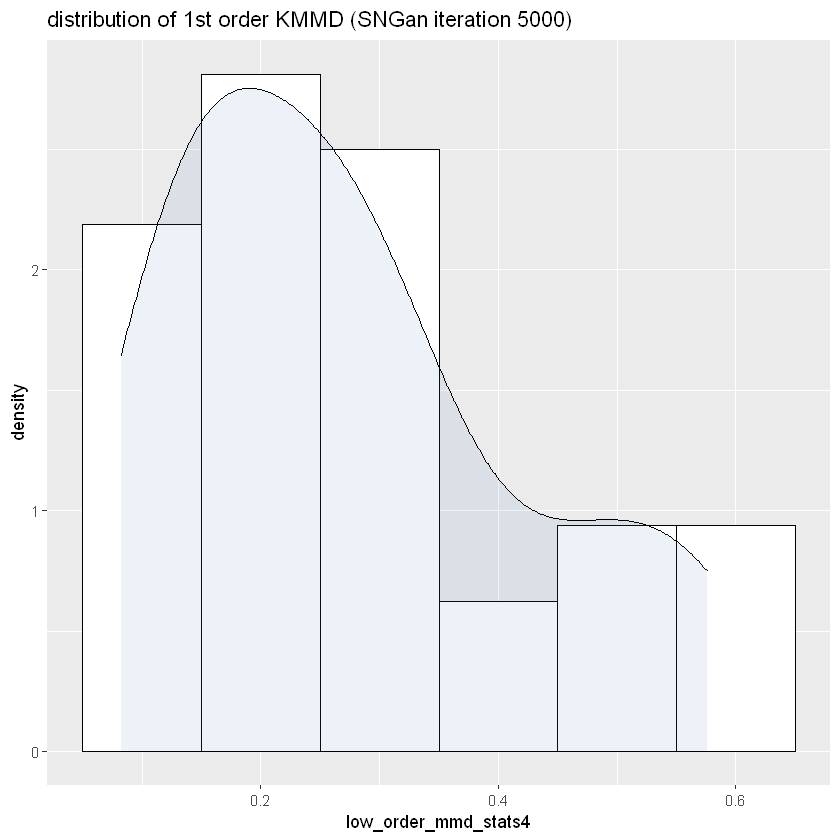
\includegraphics[width=\textwidth]{kmmd_figures/sngan_flower_lowdist_5000.png}
         \caption{5000 iterations}
     \end{subfigure}
\end{figure}

\begin{figure}[h!]
    \caption{Dataset Face}
     \centering
     \begin{subfigure}[b]{0.3\textwidth}
         \centering
         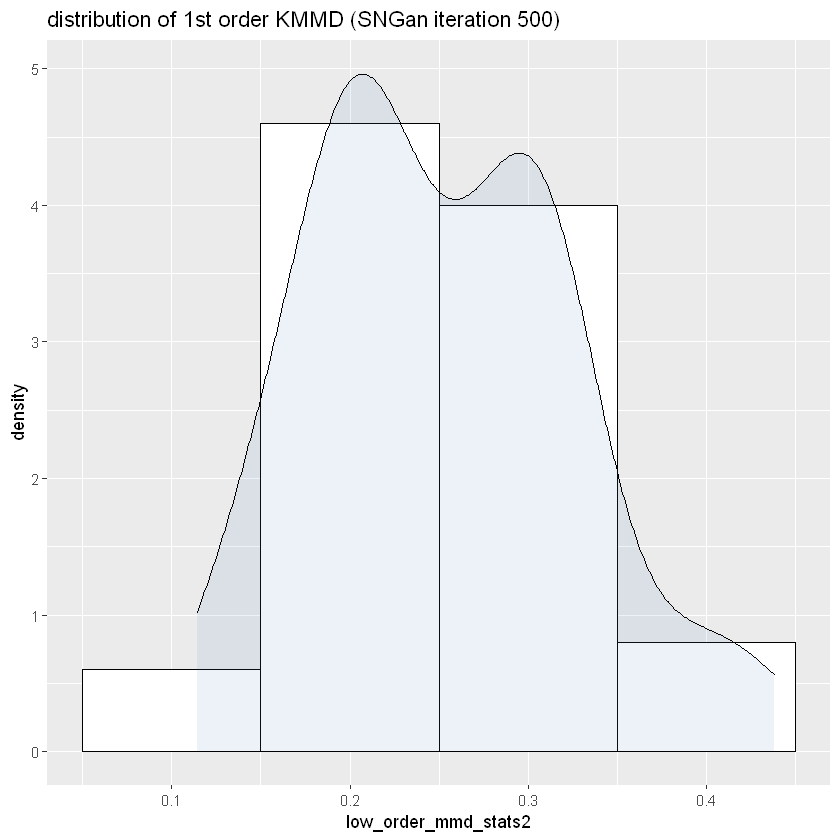
\includegraphics[width=\textwidth]{kmmd_figures/sngan_face_lowdist_500.png}
         \caption{500 iterations}
     \end{subfigure}
     \hfill
     \begin{subfigure}[b]{0.3\textwidth}
         \centering
         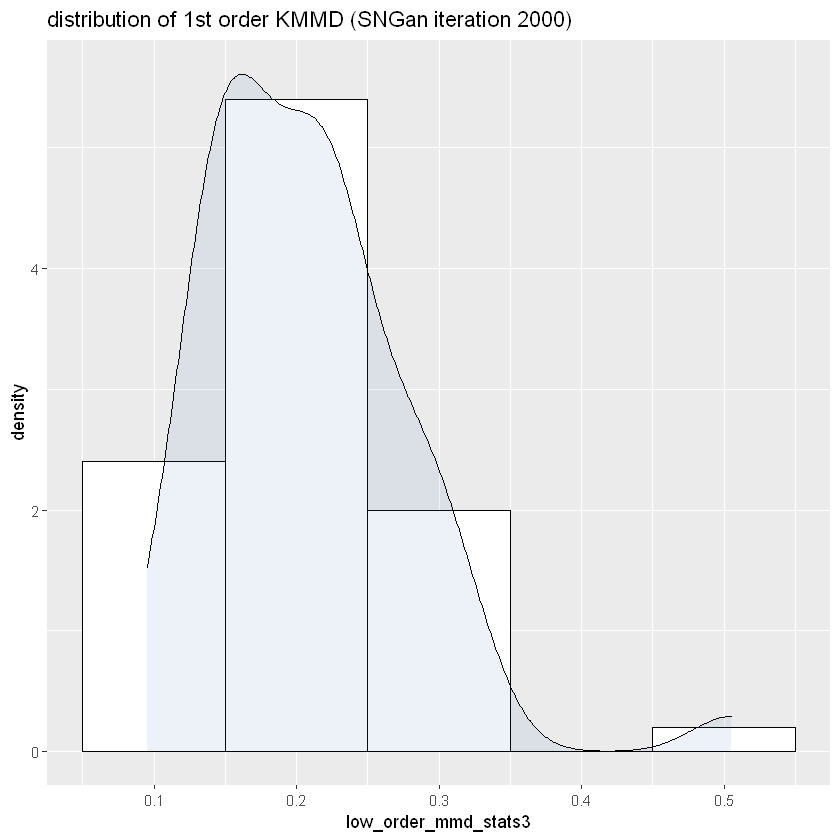
\includegraphics[width=\textwidth]{kmmd_figures/sngan_face_lowdist_2000.png}
         \caption{2000 iterations}
     \end{subfigure}
     \hfill
     \begin{subfigure}[b]{0.3\textwidth}
         \centering
         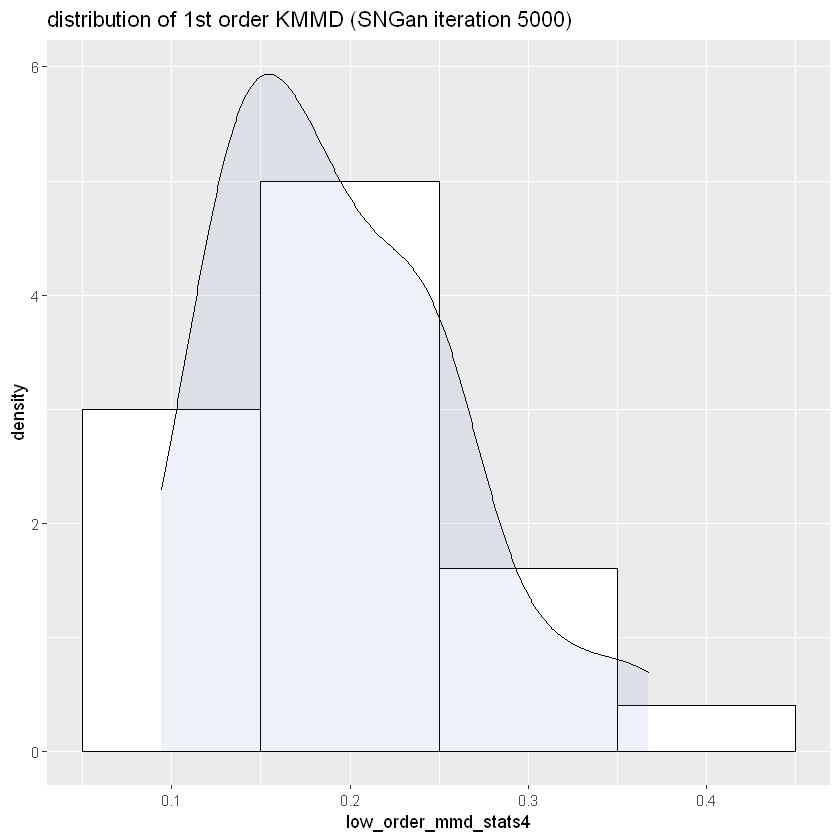
\includegraphics[width=\textwidth]{kmmd_figures/sngan_face_lowdist_5000.png}
         \caption{5000 iterations}
     \end{subfigure}
\end{figure}

\begin{figure}[h!]
    \caption{Dataset Anime}
     \centering
     \begin{subfigure}[b]{0.3\textwidth}
         \centering
         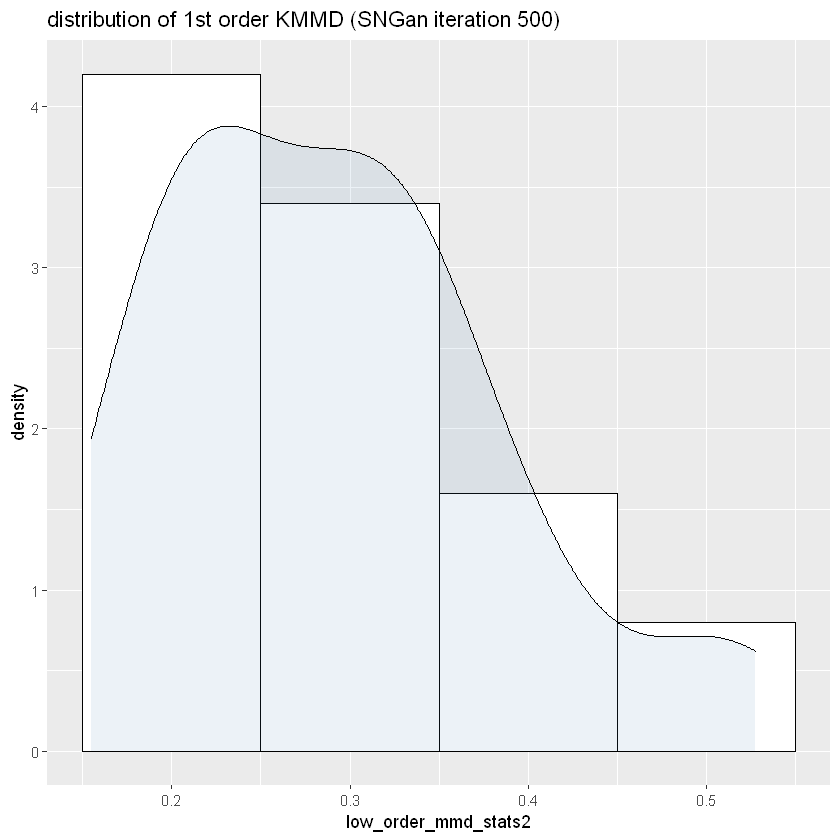
\includegraphics[width=\textwidth]{kmmd_figures/sngan_anime_lowdist_500.png}
         \caption{500 iterations}
     \end{subfigure}
     \hfill
     \begin{subfigure}[b]{0.3\textwidth}
         \centering
         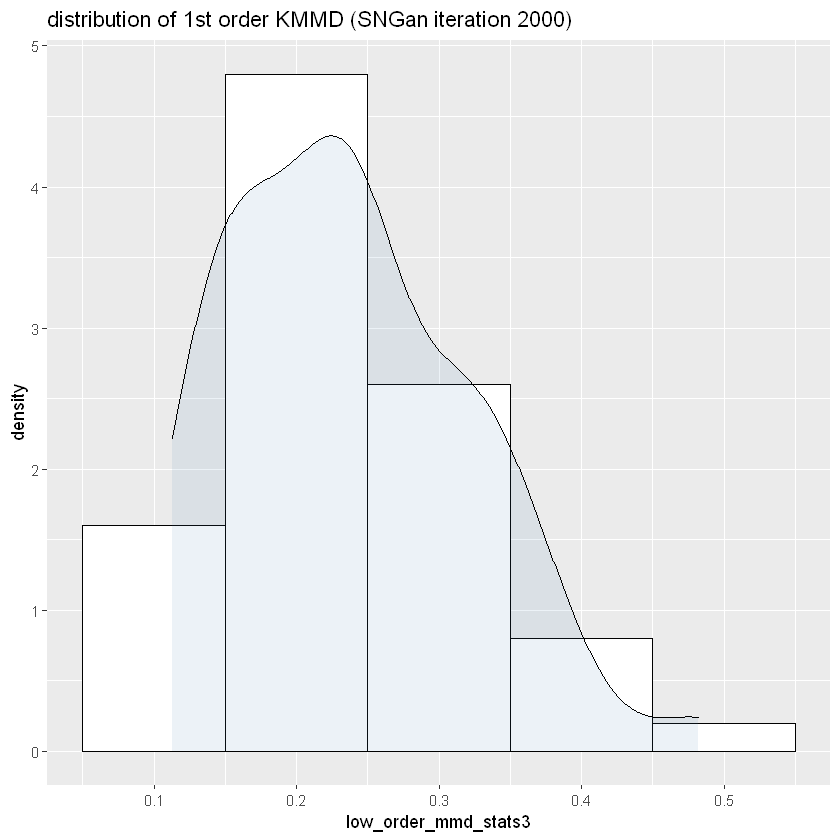
\includegraphics[width=\textwidth]{kmmd_figures/sngan_anime_lowdist_2000.png}
         \caption{2000 iterations}
     \end{subfigure}
     \hfill
     \begin{subfigure}[b]{0.3\textwidth}
         \centering
         \includegraphics[width=\textwidth]{kmmd_figures/sngan_anime_lowdist_5000.png}
         \caption{5000 iterations}
     \end{subfigure}
\end{figure}

\newpage
\subsection*{KMMD first order test statistics distribution for BigGAN}
\begin{figure}[h!]
    \caption{Dataset Flower}
     \centering
     \begin{subfigure}[b]{0.3\textwidth}
         \centering
         \includegraphics[width=\textwidth]{kmmd_figures/biggan_flower_lowdist_500.png}
         \caption{500 iterations}
     \end{subfigure}
     \hfill
     \begin{subfigure}[b]{0.3\textwidth}
         \centering
         \includegraphics[width=\textwidth]{kmmd_figures/biggan_flower_lowdist_2000.png}
         \caption{2000 iterations}
     \end{subfigure}
     \hfill
     \begin{subfigure}[b]{0.3\textwidth}
         \centering
         \includegraphics[width=\textwidth]{kmmd_figures/biggan_flower_lowdist_5000.png}
         \caption{5000 iterations}
     \end{subfigure}
\end{figure}

\begin{figure}[h!]
    \caption{Dataset Face}
     \centering
     \begin{subfigure}[b]{0.3\textwidth}
         \centering
         \includegraphics[width=\textwidth]{kmmd_figures/biggan_face_lowdist_500.png}
         \caption{500 iterations}
     \end{subfigure}
     \hfill
     \begin{subfigure}[b]{0.3\textwidth}
         \centering
         \includegraphics[width=\textwidth]{kmmd_figures/biggan_face_lowdist_2000.png}
         \caption{2000 iterations}
     \end{subfigure}
     \hfill
     \begin{subfigure}[b]{0.3\textwidth}
         \centering
         \includegraphics[width=\textwidth]{kmmd_figures/biggan_face_lowdist_5000.png}
         \caption{5000 iterations}
     \end{subfigure}
\end{figure}

\begin{figure}[h!]
    \caption{Dataset Anime}
     \centering
     \begin{subfigure}[b]{0.3\textwidth}
         \centering
         \includegraphics[width=\textwidth]{kmmd_figures/biggan_anime_lowdist_500.png}
         \caption{500 iterations}
     \end{subfigure}
     \hfill
     \begin{subfigure}[b]{0.3\textwidth}
         \centering
         \includegraphics[width=\textwidth]{kmmd_figures/biggan_anime_lowdist_2000.png}
         \caption{2000 iterations}
     \end{subfigure}
     \hfill
     \begin{subfigure}[b]{0.3\textwidth}
         \centering
         \includegraphics[width=\textwidth]{kmmd_figures/biggan_anime_lowdist_5000.png}
         \caption{5000 iterations}
     \end{subfigure}
\end{figure}

\pagebreak
\subsection*{KMMD third order test statistics distribution for SNGAN}
\begin{figure}[h!]
    \caption{Dataset Flower}
     \centering
     \begin{subfigure}[b]{0.3\textwidth}
         \centering
         \includegraphics[width=\textwidth]{kmmd_figures/sngan_flower_highdist_500.png}
         \caption{500 iterations}
     \end{subfigure}
     \hfill
     \begin{subfigure}[b]{0.3\textwidth}
         \centering
         \includegraphics[width=\textwidth]{kmmd_figures/sngan_flower_highdist_2000.png}
         \caption{2000 iterations}
     \end{subfigure}
     \hfill
     \begin{subfigure}[b]{0.3\textwidth}
         \centering
         \includegraphics[width=\textwidth]{kmmd_figures/sngan_flower_highdist_5000.png}
         \caption{5000 iterations}
     \end{subfigure}
\end{figure}

\begin{figure}[h!]
    \caption{Dataset Face}
     \centering
     \begin{subfigure}[b]{0.3\textwidth}
         \centering
         \includegraphics[width=\textwidth]{kmmd_figures/sngan_face_highdist_500.png}
         \caption{500 iterations}
     \end{subfigure}
     \hfill
     \begin{subfigure}[b]{0.3\textwidth}
         \centering
         \includegraphics[width=\textwidth]{kmmd_figures/sngan_face_highdist_2000.png}
         \caption{2000 iterations}
     \end{subfigure}
     \hfill
     \begin{subfigure}[b]{0.3\textwidth}
         \centering
         \includegraphics[width=\textwidth]{kmmd_figures/sngan_face_highdist_5000.png}
         \caption{5000 iterations}
     \end{subfigure}
\end{figure}

\begin{figure}[h!]
    \caption{Dataset Anime}
     \centering
     \begin{subfigure}[b]{0.3\textwidth}
         \centering
         \includegraphics[width=\textwidth]{kmmd_figures/sngan_anime_highdist_500.png}
         \caption{500 iterations}
     \end{subfigure}
     \hfill
     \begin{subfigure}[b]{0.3\textwidth}
         \centering
         \includegraphics[width=\textwidth]{kmmd_figures/sngan_anime_highdist_2000.png}
         \caption{2000 iterations}
     \end{subfigure}
     \hfill
     \begin{subfigure}[b]{0.3\textwidth}
         \centering
         \includegraphics[width=\textwidth]{kmmd_figures/sngan_anime_highdist_5000.png}
         \caption{5000 iterations}
     \end{subfigure}
\end{figure}

\pagebreak
\subsection*{KMMD third order test statistics distribution for BigGAN}
\begin{figure}[h!]
    \caption{Dataset Flower}
     \centering
     \begin{subfigure}[b]{0.3\textwidth}
         \centering
         \includegraphics[width=\textwidth]{kmmd_figures/biggan_flower_highdist_500.png}
         \caption{500 iterations}
     \end{subfigure}
     \hfill
     \begin{subfigure}[b]{0.3\textwidth}
         \centering
         \includegraphics[width=\textwidth]{kmmd_figures/biggan_flower_highdist_2000.png}
         \caption{2000 iterations}
     \end{subfigure}
     \hfill
     \begin{subfigure}[b]{0.3\textwidth}
         \centering
         \includegraphics[width=\textwidth]{kmmd_figures/biggan_flower_highdist_5000.png}
         \caption{5000 iterations}
     \end{subfigure}
\end{figure}

\begin{figure}[h!]
    \caption{Dataset Face}
     \centering
     \begin{subfigure}[b]{0.3\textwidth}
         \centering
         \includegraphics[width=\textwidth]{kmmd_figures/biggan_face_highdist_500.png}
         \caption{500 iterations}
     \end{subfigure}
     \hfill
     \begin{subfigure}[b]{0.3\textwidth}
         \centering
         \includegraphics[width=\textwidth]{kmmd_figures/biggan_face_highdist_2000.png}
         \caption{2000 iterations}
     \end{subfigure}
     \hfill
     \begin{subfigure}[b]{0.3\textwidth}
         \centering
         \includegraphics[width=\textwidth]{kmmd_figures/biggan_face_highdist_5000.png}
         \caption{5000 iterations}
     \end{subfigure}
\end{figure}

\begin{figure}[h!]
    \caption{Dataset Anime}
     \centering
     \begin{subfigure}[b]{0.3\textwidth}
         \centering
         \includegraphics[width=\textwidth]{kmmd_figures/biggan_anime_highdist_500.png}
         \caption{500 iterations}
     \end{subfigure}
     \hfill
     \begin{subfigure}[b]{0.3\textwidth}
         \centering
         \includegraphics[width=\textwidth]{kmmd_figures/biggan_anime_highdist_2000.png}
         \caption{2000 iterations}
     \end{subfigure}
     \hfill
     \begin{subfigure}[b]{0.3\textwidth}
         \centering
         \includegraphics[width=\textwidth]{kmmd_figures/biggan_anime_highdist_5000.png}
         \caption{5000 iterations}
     \end{subfigure}
\end{figure}

\end{document}